% mlr3fairness currently has two preprocessing methods, one postprocessing method and several fairness adjusted models implemented. We decide to use a reweighing methods that works with assigning weights to the observations to equalise the distribution of $P(Y|PA)$.
% The inprocessing method is a fairness-adjusted logistic regression implemented in mlr3fairness inspired by Zafar et. al. This method optimises for statistical parity (independence). The postprocessing method we choose aims for equalised odds and it works by randomly flipping a subset of predictions with pre-computed probabilities in order to satisfy equalised odds constraints.
\subsubsection*{Bias and the feedback loop}
\begin{figure}
    \centering
    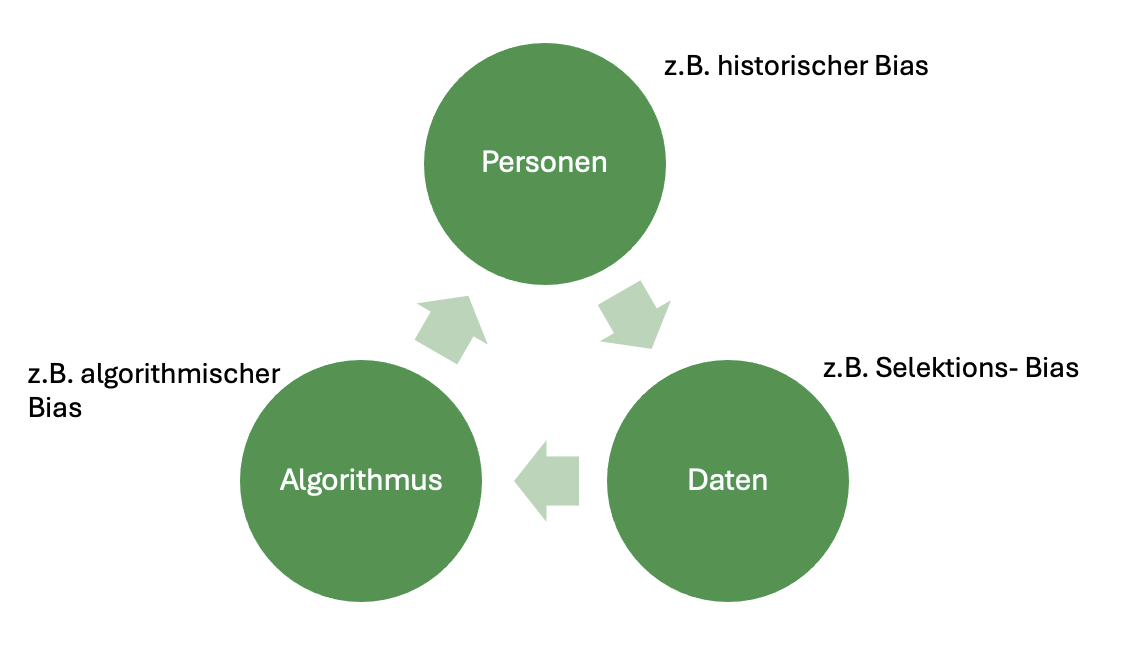
\includegraphics[width=0.7\textwidth]{../figures/bias_loop.png}
    \caption{The bias loop.}
    \label{fig:bias_loop}
\end{figure}

Usually fairness is a concern in the first place, because the algorithm should be implemented as an ADM to assist decision-making in some way. As such it could influence if someone gets admitted to college, gets a loan or is released from prison. The algorithm does not exist in isolation, but is embedded in a loop with data and the user.
We make the circumstances of a decision measurable by collecting data. The algorithm learns from this data to make an optimal prediction, on which the decision-makers base their judgement on \autoref{fig:bias_loop}. At each step of this loop, bias can be introduced in the process and, more dangerous, be amplified as the algorithm influences decision-making on a large scale.
This means that every fairness project comes with the task to understand where the data comes from and how exactly the algorithm will be deployed in practice. Let us therefore take a step back and look at the context of the SQF data.



Problem of Inframarginality \cite{corbett-davies}
"In this example, the incompatibility between threshold policies and classification parity stems from the fact that
the risk distributions differ across groups. This general phenomenon is known as the problem of inframarginality in
the economics and statistics literature, and has long been known to plague tests of discrimination in human decisions"
For our case this would mean the risk of risk of the target (of being arrested, of being searched, of having a weapon)
is really not the same for all groups in the true populaiton. This is realistic and is to be assumed. THen \cite{corbett-davies}
argues that group fairness will no lead to individual fairness, and the optimal classifier from a utility maximazation perspective
for the individual will not be fair for the group.

In case of SQF, the observed crime rate among african americans is higher (according to official statistics from NYPD).
So it would make sense that more african americans are stopped because they have higher risk scores in general. But the higher risk
scores for african americams should be questioned in the first place. They are of course not due to the fact that african americans
are truly more likely to committ crime in the first place, but they have developed over many centuries of racial discrimination
and targeted policing (lower socio-economic status and more repoerted crime rates because more polcie in these regions).
So in this dataset we basically have the problem that
- risk scores in the ture population are really different (african americans higher crime rate than white people) $\rightarrow$ due to historical bias, no objective truth process
- do not know yet whether risk scores (a.k.a. crime rate) is higher for african americans in my sample
- could be that the crime rate in sample is distributed in the same way as in the true population (african americans have higher crime rate than white people)
- could be that the crime rate in sample is distributed in a different way than in the true population (african americans have lower crime rate than white people)
$\rightarrow$this would be the extreme strict effect described in \cite{kallus2018} where the stop decision is so
biased that we explicitly target innocent african americans (this is likely not the case)

This ties into the comment in \cite{castelnovo2022} that Separation is appropriate when
the true lable $Y$ is an objective truth. Here at first sight we would say, whether someone
has commited a crime or not is an objective truth. But in reality, the fact that someone committed
a crime is influenced by historic bias.
Then enfrocing statistical parity here would be good ?? No because then this would e.g. lead
to many innocent white people being wrongly accused of crime because after all at the present white people
commit less crimes than african americans.


The story I actually want to tell in the end is that hey this is what our results show. It is not a super clear picture and maybe not what you expect, but to see the situation here clearly we have to take into account historical bias ("infected" Y) and sampling bias (PoC more easily stopped). Historical bias currently no specific method or idea to show it, sampling bias is addressed in the literature e.g. simulating the target population with weighing method.




